\newpage
\chapter{DOCUMENTO DE PROJETO}\label{apendice_projeto}

\section{Introdução}
Este documento é o plano de projeto para o AskMath, ele será usado para 
gerenciar a execução projeto. Nele, está contido os planos de gerenciamento de 
pessoal, riscos e o cronograma geral que será usado para executar cada atividade 
necessária para desenvolver o sistema.

\section{Proposito}
Esse documento foi desenvolvido para facilitar o acompanhamento do projeto 
pelos interessados, ele será utilizado durante o projeto, as revisões, as 
verificações 
até a entrega e aceitação final do produto pelo cliente, conforme acontecer o 
avanço no ciclo de vida do projeto, esse documento poderá ser atualizado para 
comportar as mudanças que venha ocorrer.

\section{Público Alvo}
Esse projeto é voltado para o Cliente que solicitou o produto como também para 
toda a equipe de desenvolvimento, para assim, facilitar o entendimento do 
processo em que o produto será desenvolvido.

\section{Evolução do Plano de Projeto}
Esse plano de projeto estará em constante mudança, a medida que o projeto for 
sendo utilizado pela equipe, novas e melhores formas de se gerenciar poderão vir 
a aparecer, acarretando assim numa atualização do projeto atual.

\section{Visão geral do Projeto}
\subsection{Necessidades do Cliente}

\begin{table}[H]
\centering
\caption{Nescessidades do Cliente}
\label{table_nescessidades_cliente}
\resizebox{\textwidth}{!}{
\begin{tabular}{|l|l|}
\hline
\multicolumn{2}{|c|}{Nescessidades do Cliente} \\ \hline
NEC01 & O Cliente necessita fornecer aos seus alunos uma ferramenta onde eles 
possam utilizar para quantificar seu nível de conhecimento. \\ \hline
NEC02 & O Cliente necessita que a ferramenta gere relatórios que mostrem o 
andamento dos alunos na ferramenta. \\ \hline
NEC03 & Na ferramenta, deve existir um fórum anônimo onde os alunos possam expor 
suas duvidas para que outros alunos posam lhes ajudar. \\ \hline
\end{tabular}}
\end{table}

\subsection{Escopo do Projeto}
O Sistema AskMath proposto pelo PETTI, tem por objetivo auxiliar no aprendizado 
dos alunos da disciplina de Matemática Básica, dispondo de um ambiente de estudo 
em que o aluno possa aprender de forma simples e intuitiva, além de compartilhar 
suas duvidas com outros alunos e professores para obter ajuda o mais rápido 
possível. Do sistema, o professor também deve obter relatórios do andamentos dos 
alunos para poder assim, adaptar suas metodologias de ensino no decorrer da 
disciplinas.

\section{Gerenciamento de Riscos}
Nessa seção, apresentaremos as formas como iremos abordar, planejar e executar 
as atividades para esse projeto.

\subsection{Metodologia}

A metodologia adotada será um processo iterativo que continua ao longo do 
desenvolvimento do projeto. Um plano de gerenciamento de ricos inicial será 
elaborado, onde este vai ser monitorado para detectar a possibilidade de riscos 
emergentes. A obtenção de mais informações de riscos é realizada durante o 
processo de desenvolvimento do plano de projeto e do projeto, caso as 
informações estejam disponíveis, os riscos serão reavaliados e será verificado 
se sua prioridade de risco mudou.

O Diagrama do processo de desenvolvimento de risco pode ser encontrado na 
\autoref{figura_processo_riscos}

\begin{figure}[H]
\centering
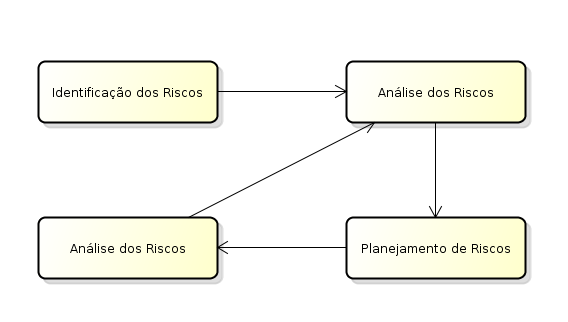
\includegraphics[width=10cm]{figuras/figura_processo_riscos}
\caption{Processo utilizado para gerenciar os riscos}
\label{figura_processo_riscos}
\end{figure}

\subsubsection{Identificação de Riscos}
A Identificação de Riscos diz respeito à identificação de riscos que podem 
representar uma ameaça para o processo de desenvolvimento de software, o 
software que esta sendo desenvolvido ou a organização de desenvolvimento. Um 
checklist de tipos diferentes de ricos será utilizado para uma identificação 
inicial dos ricos. Este estágio do processo gera uma lista de potenciais ricos, 
estes ricos podem ser encontrados na \autoref{table_riscos_encontrados}.

\begin{table}[H]
\centering
\caption{Riscos Encontrados}
\label{table_riscos_encontrados}

\resizebox{\textwidth}{!}{
\begin{tabular}{|l|l|}
\hline
\multicolumn{1}{|c|}{\textbf{Tipo de riscos}} & 
\multicolumn{1}{c|}{\textbf{Possíveis Riscos}} \\ \hline
Tecnologia & \begin{tabular}[c]{@{}l@{}}Atrasos de especificação (1)\\ Mudança 
de tecnologia (2)\\ Componentes reusáveis não atendem as especificações (3)\\ 
Problema para Integrar os Modulos (4)\end{tabular} \\ \hline
Pessoas & Pessoas estão doentes (5) \\ \hline
Organizacional & O produto fere principios da intituição (6) \\ \hline
Ferramentas & \begin{tabular}[c]{@{}l@{}}Ferramentas são difíceis de serem 
utilizadas (7)\\ Dificuldade na instalação das ferramentas (8)\end{tabular} \\ 
\hline
Requisitos & \begin{tabular}[c]{@{}l@{}}Mudança de requisitos que requerem 
retrabalho do projeto(9)\\ O Cliente não possui tempo livre para se reunir 
pessoalmente com a equipe (10)\end{tabular} \\ \hline
Estimativa & \begin{tabular}[c]{@{}l@{}}Tamanho do software subestimado (11)\\ 
Atrasos no Cronograma (12)\\ A taxa de reparo de defeito é substimado 
(13)\end{tabular} \\ \hline
\end{tabular}}
\end{table}


\subsubsection{Análise de Riscos}
Nesta fase do processo cada risco identificado na etapa 
anterior é analisado e classificado sobre a probabilidade de riscos e seu 
impacto no projeto caso ocorra (As definições de probabilidade e impacto de 
risco se encontra em dos tópicos seguintes). Uma vez analisados e classificados 
os riscos mais significativos serão identificados e estes serão riscos que vão 
ser monitorados durando o projeto.

Este estágio do processo gera uma lista de prioridade de riscos, esta lista se 
encontra na \autoref{table_lista_prioridade_riscos}.

\begin{table}[H]
\centering
\caption{Lista de Prioridade dos Riscos}
\label{table_lista_prioridade_riscos}
\resizebox{\textwidth}{!}{
\begin{tabular}{|l|l|l|l|}
\hline
\multicolumn{1}{|c|}{\textbf{Risco}} & 
\multicolumn{1}{c|}{\textbf{Probabilidade}} & 
\multicolumn{1}{c|}{\textbf{Efeito}} & \multicolumn{1}{c|}{\textbf{Afeta}} \\ 
\hline
Atrasos de especificação (1) & Quase Certo & Médio & Projeto e Produto \\ \hline
Mudança de tecnologia (2) & Pouco Provável & Muito Alto & Projeto e Produto \\ 
\hline
Componentes reusáveis não atendem as especificações (3) & Pouco Provável & Muito 
Alto & Projeto \\ \hline
Problema para Integrar os Módulos (4) & Pouco Provável & Alto & Produto \\ 
\hline
Pessoas estão doentes (5) & Raro & Baixo & Organização \\ \hline
O produto fere princípios da instituição (6) & Improvável & Alto & Produto \\ 
\hline
Ferramentas são difíceis de serem utilizadas (7) & Pouco Provável & Médio & 
Projeto \\ \hline
Dificuldade na instalação das ferramentas (8) & Pouco Provável & Médio & Projeto 
\\ \hline
Mudança de requisitos que requerem retrabalho do projeto(9) & Pouco Provável & 
Muito Alto & Projeto e Produto \\ \hline
O Cliente não possui tempo livre para se reunir pessoalmente com a equipe (10) & 
Muito Provável & Médio & Projeto \\ \hline
Tamanho do software subestimado (11) & Quase Certo & Médio & Projeto \\ \hline
Atrasos no Cronograma (12) & Quase Certo & Baixo & Projeto \\ \hline
A taxa de reparo de defeito é subestimado (13) & Quase Certo & Baixo & Projeto e 
Produto \\ \hline
\end{tabular}}
\end{table}

\subsubsection{Planejamento dos Riscos}

O Planejamento dos riscos, considera cada um dos riscos que foram identificados 
e desenvolve estratégias para gerenciar estes ricos. Este estágio do processo 
gera uma lista de prevenção de riscos e planos de contingência, esta lista pode 
ser encontrada na \autoref{table_lista_prevencao_contigencia}.

\begin{table}[H]
\centering
\caption{Lista Prevenção de Riscos e Planos de Contingência}
\label{table_lista_prevencao_contigencia}
\resizebox{\textwidth}{!}{
\begin{tabular}{|l|l|}
\hline
\multicolumn{1}{|c|}{\textbf{Risco}} & \multicolumn{1}{c|}{\textbf{Estratégia}} 
\\ \hline
Atrasos de especificação (1) & Componentes e requisitos que são pré-requisitos 
de outros possuem seus desenvolvimentos adiantados. \\ \hline

Mudança de tecnologia (2) & As tecnologias a serem utilizadas são analizadas e 
avaliadas antes de serem usadas para evitar possíveis mudanças. Uma tecnologia 
reserva deve ser escolhida em caso de eventual mudança não prevista. \\ \hline

Problema para Integrar os Módulos (4) & Os módulos serão desenvolvidos pensando 
em como integra-los futuramente, usando algum modelo de desenvolvimento, como 
MVC ou Camadas. Em caso de módulos externos bibliotecas que fazem a comunicação 
terão de ser criadas (aumento de custo e possível atraso no cronograma). \\ 
\hline

O produto fere princípios da instituição (6) & Estudar as normas da instituição 
e desenvolver o software dentro delas. \\ \hline

Ferramentas são difíceis de serem utilizadas (7) & Estar sempre se comunicando 
com o usuário em cada fase de desenvolvimento para o recebimento de feedbacks, 
evitando mudanças drásticas em etapas finais do projeto. \\ \hline

Mudança de requisitos que requerem retrabalho do projeto(9) & Estar sempre se 
comunicando com o usuário em cada fase de desenvolvimento para o recebimento de 
feedbacks, evitando mudanças drásticas em etapas finais do projeto. \\ \hline

A taxa de reparo de defeito é subestimado (13) & Avaliar o defeito antes de 
estimular seu reparo. \\ \hline
\end{tabular}}
\end{table}

\subsubsection{Monitoração de riscos}

O Monitoração de riscos verifica se as suposições definidas sobre os riscos 
não foram alteradas durante o processo de desenvolvimento do projeto. Para isso 
são avaliados os outros fatores que dão a probabilidade de riscos e seus 
efeitos. Este estágio de processo gera a tabela de avaliação de riscos.